\documentclass[tikz,border=10pt]{standalone}
\usepackage[T1]{fontenc}
\usepackage{lmodern}
\usepackage{amsmath,amssymb}
\usetikzlibrary{arrows.meta,positioning,fit,backgrounds}

\definecolor{inkblack}{HTML}{141416}
\definecolor{slateink}{HTML}{334155}
\definecolor{navyfill}{HTML}{2B3A67}
\definecolor{plumfill}{HTML}{5B3E6B}
\definecolor{amberfill}{HTML}{B45309}
\definecolor{softbg}{HTML}{F8FAFC}

\begin{document}
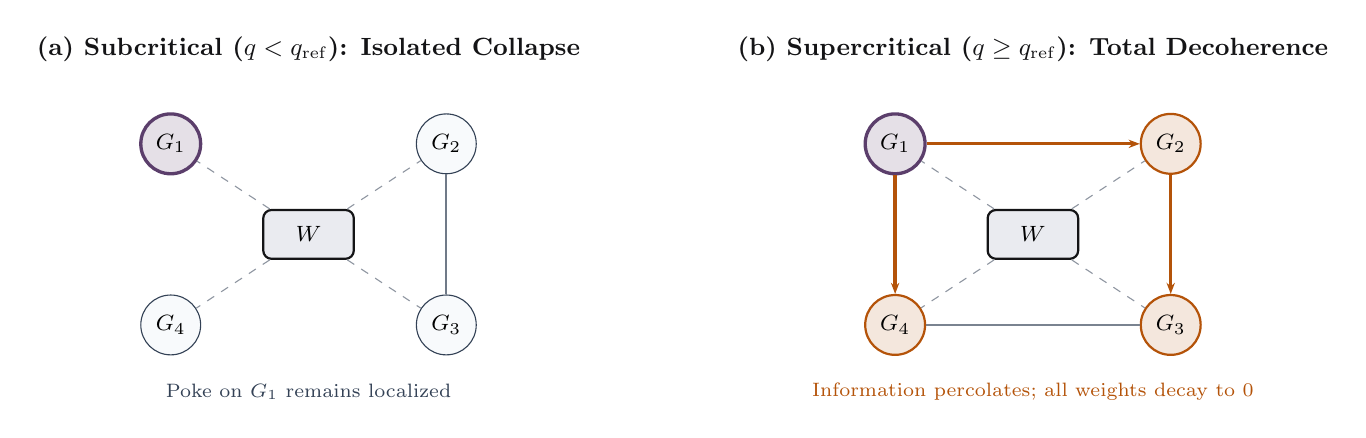
\begin{tikzpicture}[
  font=\small,
  node/.style={circle, draw=slateink, fill=softbg, minimum size=0.76cm, inner sep=1pt, font=\footnotesize\bfseries},
  poked/.style={circle, draw=plumfill, very thick, fill=plumfill!16, minimum size=0.76cm, inner sep=1pt, font=\footnotesize\bfseries},
  informed/.style={circle, draw=amberfill, thick, fill=amberfill!14, minimum size=0.76cm, inner sep=1pt, font=\footnotesize\bfseries},
  focal/.style={rectangle, rounded corners=3pt, draw=inkblack, thick, fill=navyfill!10, minimum width=1.15cm, minimum height=0.62cm, font=\footnotesize\bfseries}
]

% Left panel: Subcritical (sparse friend graph)
\node[font=\bfseries\small, inkblack] at (0, 2.35) {(a) Subcritical ($q < q_{\mathrm{ref}}$): Isolated Collapse};
\node[focal] (W1) at (0, 0) {$W$};
\node[poked] (A1) at (-1.75, 1.15) {$G_1$};
\node[node]  (A2) at (1.75, 1.15)  {$G_2$};
\node[node]  (A3) at (1.75, -1.15) {$G_3$};
\node[node]  (A4) at (-1.75, -1.15){$G_4$};

\draw[slateink!55, dashed] (W1) -- (A1);
\draw[slateink!55, dashed] (W1) -- (A2);
\draw[slateink!55, dashed] (W1) -- (A3);
\draw[slateink!55, dashed] (W1) -- (A4);
\draw[slateink!70, thick] (A2) -- (A3);
\node[font=\scriptsize\color{slateink}] at (0, -2.0) {Poke on $G_1$ remains localized};

% Right panel: Supercritical (connected friend graph) with clean horizontal separation
\begin{scope}[xshift=9.2cm]
\node[font=\bfseries\small, inkblack] at (0, 2.35) {(b) Supercritical ($q \ge q_{\mathrm{ref}}$): Total Decoherence};
\node[focal] (W2) at (0, 0) {$W$};
\node[poked]    (B1) at (-1.75, 1.15) {$G_1$};
\node[informed] (B2) at (1.75, 1.15)  {$G_2$};
\node[informed] (B3) at (1.75, -1.15) {$G_3$};
\node[informed] (B4) at (-1.75, -1.15){$G_4$};

\draw[slateink!55, dashed] (W2) -- (B1);
\draw[slateink!55, dashed] (W2) -- (B2);
\draw[slateink!55, dashed] (W2) -- (B3);
\draw[slateink!55, dashed] (W2) -- (B4);

\draw[amberfill, very thick, -{Stealth[length=4pt]}] (B1) -- (B2);
\draw[amberfill, very thick, -{Stealth[length=4pt]}] (B2) -- (B3);
\draw[amberfill, very thick, -{Stealth[length=4pt]}] (B1) -- (B4);
\draw[slateink!65, thick] (B3) -- (B4);
\node[font=\scriptsize\color{amberfill}] at (0, -2.0) {Information percolates; all weights decay to $0$};
\end{scope}

\end{tikzpicture}
\end{document}
